%; whizzy document
% latex beamer presentation.
% platex, latex-beamer でコンパイルすることを想定。 

%     Tokyo Debian Meeting resources
%     Copyright (C) 2006 Junichi Uekawa

%     This program is free software; you can redistribute it and/or modify
%     it under the terms of the GNU General Public License as published by
%     the Free Software Foundation; either version 2 of the License, or
%     (at your option) any later version.

%     This program is distributed in the hope that it will be useful,
%     but WITHOUT ANY WARRANTY; without even the implied warranty of
%     MERCHANTABILITY or FITNESS FOR A PARTICULAR PURPOSE.  See the
%     GNU General Public License for more details.

%     You should have received a copy of the GNU General Public License
%     along with this program; if not, write to the Free Software
%     Foundation, Inc., 51 Franklin St, Fifth Floor, Boston, MA  02110-1301 USA

% 実行順番
% sudo  ~/bin/usb-macbook-ir.c &
% real presentation (shell-command (concat "DISPLAY=:0.1 xpdf -fullscreen " (replace-regexp-in-string "tex$" "pdf"(buffer-file-name)) "&"))
% DISPLAY=:0.1 xpdf -fullscreen 

\documentclass[cjk,dvipdfmx]{beamer}
\usetheme{Warsaw}
%  preview (shell-command (concat "xpdf " (replace-regexp-in-string "tex$" "pdf"(buffer-file-name)) "&"))
%  presentation (shell-command (concat "xpdf -fullscreen " (replace-regexp-in-string "tex$" "pdf"(buffer-file-name)) "&"))

%http://www.naney.org/diki/dk/hyperref.html
%日本語EUC系環境の時
\AtBeginDvi{\special{pdf:tounicode EUC-UCS2}}
%シフトJIS系環境の時
%\AtBeginDvi{\special{pdf:tounicode 90ms-RKSJ-UCS2}}

\title{東京エリア Debian 勉強会}
\subtitle{資料}
\author{上川 純一 dancer@debian.org\\IRC nick: dancerj}
\date{2006年10月21日}
\logo{
\includegraphics[width=8cm]{image200607/openlogo-light.eps}}

% 三択問題用
\newcounter{santakucounter}
\newcommand{\santaku}[5]{%
\addtocounter{santakucounter}{1}
\frame{\frametitle{問題\arabic{santakucounter}. #1}
%問題\arabic{santakucounter}. #1
\begin{minipage}[t]{0.7\hsize}
 \begin{itemize}
 \item  A #2\\
 \item  B #3\\
 \item  C #4\\
 \end{itemize}
\end{minipage}
}
\frame{\frametitle{問題\arabic{santakucounter}. #1}
%問題\arabic{santakucounter}. #1
\begin{minipage}[t]{0.7\hsize}
\begin{itemize}
\item  A #2\\
\item  B #3\\
\item  C #4\\
\end{itemize}
\end{minipage}
\begin{minipage}[t]{0.2\hsize}
答えは:


\vspace{1cm}

{\huge \hspace{1cm}#5}
\end{minipage}}
}


\begin{document}
\frame{\titlepage{}}

\section{Intro}

\begin{frame}
 \frametitle{本日のagenda}
\begin{minipage}[t]{0.4\hsize}
  \begin{itemize}
  \item 注意事項
	\begin{itemize}
	 \item 飲食禁止
	 \item 政治/宗教/営利活動禁止
	\end{itemize}
  \item 最近事情
  \item 事前課題紹介
  \item quiz
 \end{itemize}
\end{minipage} 
\begin{minipage}[t]{0.4\hsize}
\begin{itemize}
  \item スペイン参加報告
  \item flash ねた
  \item apt チューニングねた
 \end{itemize}
\end{minipage}
\end{frame}

\section{最近のDebian関連のミーティング報告}

\begin{frame}{最近のDebian関連ミーティング報告}
 \begin{itemize}
  \item Debian勉強会
  \item 夜のカレーパーティー
  \item Debian JP 定例 IRC ミーティング試行中\\
 \end{itemize}
\end{frame}

\subsection{9月のDebian勉強会}

\begin{frame}{9月のDebian勉強会}
 \begin{itemize}
  \item あなたが知らないうちに使っているDebian specific
  \item 翻訳のすすめ
  \item dpkg, apt のプロファイリング
  \item LLGONG発表報告
 \end{itemize}
\end{frame}


\subsection{Debian JP として}

\begin{frame}{Debian JPとDebian 勉強会}
個人的な理想

\includegraphics[width=0.7\hsize]{image200610/debianstructure.eps}

\end{frame}

\section{事前課題の声}

%\subsection{}
\begin{frame}[containsverbatim]{事前課題}
\begin{verbatim}
$ cat /etc/networking/interfaces 
cat: /etc/networking/interfaces: そのようなファイルやディレクトリはありません
\end{verbatim}
\end{frame}

\begin{frame}[containsverbatim]{interfaces}
\begin{verbatim}
 iface eth0 inet dhcp
 iface eth0:1 inet static
    address 192.168.1.2
    netmask 255.255.255.0
 iface eth0:2 inet static
    address 192.168.2.2
    netmask 255.255.255.0
\end{verbatim} 
\end{frame}

\begin{frame}{ダサい}
DebianというかLinux全般の問題だと思いますが、
新しいデバイスが次々とカーネルでサポートされ、
新しいソフトウェアがどんどん開発され、
デスクトップも (まだまだという評価も否めませんが) 見違えるようにカッコよく使いやすくなっている一方で、
なんだかダサいところは誰も (興味がないのか) 手をつけずダサいままになっているような気がします。
別に設定ファイル全般が悪だとは思いませんが、
設定まわりのインタフェースはもう少し改良できるのではないでしょうか。
まぁ、だったらお前やれと言われても今の自分にはできないので、
いつかその辺りが改善されるといいですね、と無難にまとめて回答とします。
\end{frame}

\begin{frame}{設定例ほしい}

debian のネットワーク設定に関しては、マシンの用途、接続方法などでいくつ
か設定方法があると思います。私の知る限りでは以下の設定があります。


\begin{enumerate}
 \item /etc/network 以下
	interfacesとインターフェース起動時の処理のスクリプト群
 \item /etc/ppp 以下
	ppp 接続時の処理のスクリプト群
 \item dhcp 接続時
 \item network-manager を使った設定
\end{enumerate}

これらの設定の解説や設定例があるとよいとおもいます。
\end{frame}


\begin{frame}
常用のinterfacesファイルはnoauto eth0; iface eth0 inet dhcpという感じで
たいして面白いものではない。んで、Debian(およびLinux)のネットワーク設定
については不満だらけである。まず今のinterfaces+ifupdownのフォーマットが
すでに考古学博物館収録に値する代物(有史以前遺産のnetbaseよりはマシだが)
であり、CUI/GUI問わず未だにまともなセットアップツールを提供できていない。
インストーラのセットアップのほうがまだ気合いが入ってるぞ。エディタでこう
記述しろなんて言われて喜んでるのは設定オタだけで十分である。特に無線周り
は、Windows辺りと比べてしまうと、そのヘタレっぷりにDebian CDを真っ二つに
して窓から捨てたくなったとしても止めることはできないだろう。
\end{frame}

\begin{frame}
 だいたい歴史
 的負の遺産な/etc/resolv.confなんてファイルも気味が悪い。こんなのはカーネ
 ル内部に持たせてやればDHCPのときにいちいち実ファイルを書き換える必要もな
 いじゃないか。追加NICだってネットワーク接続するために付けたのであろうか
 ら、いちいちエディタでinterfacesに追記する必要なく、新しいNICデバイスを
 発見した段階でとりあえずDHCPでつなぎに行っても罰は当たらなそうなもんだ。
 まぁこういったことはデスクトップ開発者には100も承知なことなわけで、GNOME
 やKDEではネットワークマネージャソフトの開発が進んでる。Debianはどうする。
\end{frame}

\begin{frame}{みんなの思い}
\begin{itemize}
 \item VPNとの統合
 \item 無線の設定
 \item resolv.conf 
 \item 環境依存の場合のネットワーク設定
 \item 設定の一覧がわからない
 \item ipv6 がいまいち
\end{itemize}
\end{frame}


\section{DWNQuiz}
%% debianmeetingresume200609.texから以下コピー

\subsection{2006年38号}
\url{http://www.debian.org/News/weekly/2006/38/}
にある9月19日版です。

\santaku
{Josselin Mouette が GNOME 2.16 について説明したのは}
{stable へのバックポート}
{experimental への投入}
{unstable への投入}
{B}

\santaku
{Russel Coker が議論する際の道具として提案したのは?}
{意味の無い議論をベイジアンフィルタではじく}
{killfile の積極的な活用}
{議論のサマリをまとめるためのwikiの利用}
{C}

\santaku
{最近 Debian にはいったパッケージである「ttf-vlgothic」のvlはどういう意味か?}
{ディストリビューションの名前}
{私の名前はやまねです。}
{very local }
{A}


\subsection{2006年39号}
\url{http://www.debian.org/News/weekly/2006/39/}
にある9月26日版です。

\santaku
{プロジェクトリーダーを罷免する決議が出たのはなぜか?}
{Dunk-Tank プロジェクトを発足したから}
{やるきがまったくみられないから}
{タイの政変の影響}
{A}

\santaku
{一般決議に関しての規則がかわったのはなぜか}
{現在多数提起されているから}
{くだらないものが提起されすぎだから}
{Dunk-Tank が気に入らないから}
{A}

\section{Debian勉強会 agenda}

\begin{frame}
 \frametitle{本日のagenda}
\begin{minipage}[t]{0.4\hsize}
  \begin{itemize}
  \item 注意事項
	\begin{itemize}
	 \item 飲食禁止
	 \item 政治/宗教/営利活動禁止
	\end{itemize}
  \item 最近事情
  \item 事前課題紹介
  \item quiz
 \end{itemize}
\end{minipage} 
\begin{minipage}[t]{0.4\hsize}
\begin{itemize}
  \item スペイン参加報告
  \item flash ねた
  \item apt チューニングねた
 \end{itemize}
\end{minipage}
\end{frame}

\section{aptをチューニングしてみる}

\begin{frame}
先月からつづいている aptのチューニングネタ
\end{frame}

\subsection{検討した内容}
\begin{frame}[containsverbatim]{検討した内容}
\begin{verbatim}
sudo apt-get update
[中略]
CPU: Core Solo / Duo, speed 1833 MHz (estimated)
Counted CPU_CLK_UNHALTED events (Unhalted clock cycles) with a unit mask of 0x00 (Unhalted core cycles) count 180000
samples  %        image name               app name                 symbol name
23823    46.3519  libapt-pkg-libc6.3-6.so.3.11.0 apt-get                  
SHA1Transform(unsigned int*, unsigned char const*)
12732    24.7724  libapt-pkg-libc6.3-6.so.3.11.0 apt-get
 MD5Transform(unsigned int*, unsigned int const*) 
4282      8.3314  processor.ko             processor                acpi_processor_idle
2584      5.0276  libc-2.3.6.so            apt-get                  (no symbols)
2012      3.9147  vmlinux                  vmlinux                  __copy_to_user_ll
503       0.9787  gpgv                     gpgv                     (no symbols)
222       0.4319  vmlinux                  vmlinux                  timer_interrupt
166       0.3230  libapt-pkg-libc6.3-6.so.3.11.0 apt-get
 MD5Summation::Add(unsigned char const*, unsigned long) 
\end{verbatim}
\end{frame}

\subsection{方針}
\begin{frame}{方針}
 \begin{itemize}
  \item SHA1 の計算が遅いので高速化する
 \end{itemize}
\end{frame}

\subsection{検討}
\begin{frame}{検討}
 \begin{itemize}
  \item SHA1の高速な実装を探す
  \item 既存の実装を評価
	\begin{itemize}
	 \item mozilla
	 \item openssl
	\end{itemize}
  \item 既存の実装を比較したところあまりはやくならない
 \end{itemize}
\end{frame}

\subsection{結論}
\begin{frame}{結論}
 \begin{itemize}
  \item 重い処理ではあるが、最適化されているものが既存では存在しない
  \item 高速化は自前でチューニングする必要があるらしい
  \item タイムアウト
\end{itemize}
\end{frame}

\subsection{まとめ}
\begin{frame}{まとめ}
\begin{itemize}
 \item プロファイリングすれば重い処理がわかり、
       最適化の手がかりになる
 \item 実はプロファイルを取得するのはそんなにむずかしくない
 \item みんなでアッセンブリ職人になり、最適化するしか!
\end{itemize}
\end{frame}

\subsection{今後のイベント}

\begin{frame}
 \frametitle{今後のイベント}
 \begin{itemize}
  \item OSC-Fall 10月28日?
  \item OSC 沖縄 12月1日?
  \item KOF 11月18日 
  \item Debian 勉強会大阪開催 11月19日
  \item Debian Conference 2007 Edinburgh 2007年6月
  \item Debian 14周年 2007年8月16日
  \item Debian 15周年 2008年8月16日
 \end{itemize}
\end{frame}

\section{wrap-up}
\begin{frame}
 \frametitle{今日のまとめ}
 \begin{itemize}
  \item まとめ
 \end{itemize}
\end{frame}

\end{document}
